\section{Grundlagen und Stand der Technik}

Salvaris beschreibt \textit{Machine Learning} als einen Zweig der Computerwissenschaften, bei dem Computern beigebracht wird anhand von Trainingsdaten Entscheidungen zu treffen. Typische Anwendungsgebiete des ML sind Klassifikation, Regression und Clustering. DL ist ein Teilgebiet des ML bei dem besonders komplexe Neuronale Netze mit vielen Schichten und Neuronen Verwendung finden. Ein weitere wesentliche Abgrenzung stellt die Merkmalsextraktion dar. Also die Extraktion der Eigenschaften eines Objekts, die ausschlaggebend für etwaige Klassenzugehörigkeiten sind. Diese entscheidenden Merkmale müssen dem DL-Modell nicht vorgegeben werden, sondern werden von dem Algorithmus selbst gefunden. Dieser Umstand stellt mit die größten Herausforderungen aber auch Chancen beim DL dar \cite[S.32-47]{dlazure2019}.  Im Folgenden werden nur die für die vorliegende Arbeit besonders wichtigen und speziell angepassten Methoden und Aspekte des DL erläutert. Für weiterführende grundlegende Informationen zum Beispiel zu Neuronen, Schichttypen, Aktivierungsfunktionen und zum Gradientenabstiegsverfahren wird auf \cite{dlbook2018} verwiesen.
\begin{figure}[h]\label{dlmlunterschied}
  \centering
  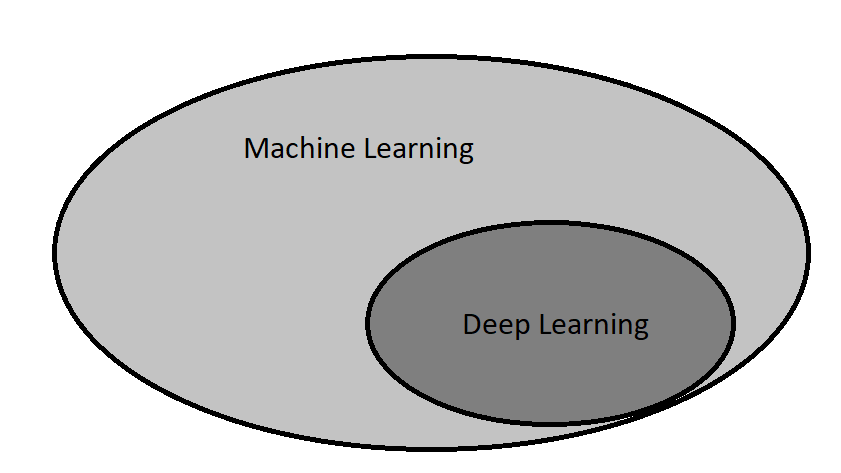
\includegraphics[width=8cm]{mldlunterschied.png}
  \caption{Abgrenzung Deep Learning zu Machine Learning.}
\end{figure}

\subsection{Convolutional Neural Networks}

\subsection{Loss-Funktionen und Metriken}